\documentclass[tikz,border=1.35mm]{standalone}

% Plain tetrahedral cell.
% The x/y/z vectors below define a fixed oblique projection for the 3D wireframe.
\begin{document}
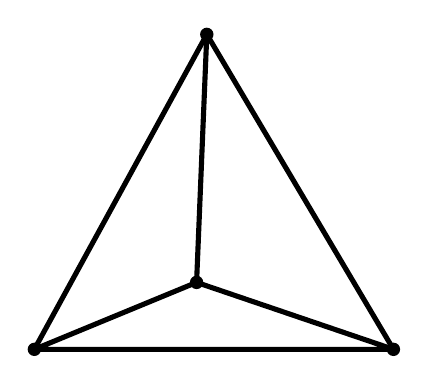
\begin{tikzpicture}[
  x={(19mm,0mm)},
  y={(7mm,4mm)},
  z={(0mm,18mm)},
  line join=round,
  line cap=round,
  edge/.style={draw=black,line width=0.65mm}
]
  % Tetrahedron vertices.
  \coordinate (v0) at (0,0,0);
  \coordinate (v1) at (2.4,0,0);
  \coordinate (v2) at (0.55,1.45,0.15);
  \coordinate (v3) at (0.95,0.55,2.1);

  % Wireframe edges.
  \draw[edge] (v0) -- (v1) -- (v2) -- cycle;
  \draw[edge] (v3) -- (v0);
  \draw[edge] (v3) -- (v1);
  \draw[edge] (v3) -- (v2);

  % Original vertices are black.
  \foreach \p in {v0,v1,v2,v3} {
    \fill[black] (\p) circle[radius=0.85mm];
  }
\end{tikzpicture}
\end{document}
